\documentclass[journal=jctc,manuscript=article]{achemso}

%%%%%%%%%%%%%%%%%%%%%%%%%%%%%%%%%%%%%%%%%%%%%%%%%%%%%%%%%%%%%%%%%%%%%
%% Place any additional packages needed here.  Only include packages
%% which are essential, to avoid problems later.
%%%%%%%%%%%%%%%%%%%%%%%%%%%%%%%%%%%%%%%%%%%%%%%%%%%%%%%%%%%%%%%%%%%%%
\usepackage{chemformula} % Formula subscripts using \ch{}
\usepackage[T1]{fontenc} % Use modern font encodings

%%%%%%%%%%%%%%%%%%%%%%%%%%%%%%%%%%%%%%%%%%%%%%%%%%%%%%%%%%%%%%%%%%%%%
%% If issues arise when submitting your manuscript, you may want to
%% un-comment the next line.  This provides information on the
%% version of every file you have used.
%%%%%%%%%%%%%%%%%%%%%%%%%%%%%%%%%%%%%%%%%%%%%%%%%%%%%%%%%%%%%%%%%%%%%
%%\listfiles

%%%%%%%%%%%%%%%%%%%%%%%%%%%%%%%%%%%%%%%%%%%%%%%%%%%%%%%%%%%%%%%%%%%%%
%% Place any additional macros here.  Please use \newcommand* where
%% possible, and avoid layout-changing macros (which are not used
%% when typesetting).
%%%%%%%%%%%%%%%%%%%%%%%%%%%%%%%%%%%%%%%%%%%%%%%%%%%%%%%%%%%%%%%%%%%%%
% \newcommand*\mycommand[1]{\texttt{\emph{#1}}}

\usepackage{fullpage}
\usepackage{amsfonts}
\usepackage{graphicx}
\usepackage{float}
\usepackage{amsmath}
\usepackage{chemfig}
\usepackage{indentfirst}
\usepackage{longtable}
\usepackage{array}
\usepackage{cellspace}
\usepackage{palatino}
%\usepackage{breqn}
\usepackage{amssymb}
\usepackage{verbatim}
\usepackage[colorlinks=true,citecolor=blue,linkcolor=blue]{hyperref}
\usepackage{siunitx}
\usepackage{xr}
%\usepackage{bibentry}
\usepackage{verbatim}

%\DefineVerbatimEnvironment%
%	{verbatimprog}%
%	{Verbatim}%
%	{fontsize=\footnotesize}%

\newenvironment{myequation}{%
\addtocounter{equation}{-1}
\refstepcounter{defcounter}
\renewcommand\theequation{SI.\thedefcounter}
\begin{equation*}}
{\end{equation*}}

\renewcommand{\thefigure}{SI.\arabic{figure}}

\renewcommand{\thepage}{SI.\arabic{page}}

\renewcommand{\thesection}{SI.\Roman{section}}

\renewcommand{\thetable}{SI.\Roman{table}}

\makeatletter
\newcommand*{\addFileDependency}[1]{% argument=file name and extension
	\typeout{(#1)}
	\@addtofilelist{#1}
	\IfFileExists{#1}{}{\typeout{No file #1.}}
}
\makeatother

\newcommand*{\myexternaldocument}[1]{%
	\externaldocument{#1}%
	\addFileDependency{#1.tex}%
	\addFileDependency{#1.aux}%
}

\myexternaldocument{H:/Publications/Postdoc_3/VLE_PVT_UA_Mie_manuscript}

\SectionNumbersOn

% The figures are in a figures/ subdirectory.
\graphicspath{{figures/}}

%\bibliographystyle{apsrevlong}
%\bibliographystyle{apsrev}
\bibliographystyle{unsrt}

% italicized boldface for math (e.g. vectors)
\newcommand{\bfv}[1]{{\mbox{\boldmath{$#1$}}}}
% non-italicized boldface for math (e.g. matrices)
\newcommand{\bfm}[1]{{\bf #1}}          

%\newcommand{\bfm}[1]{{\mbox{\boldmath{$#1$}}}}
%\newcommand{\bfm}[1]{{\bf #1}}
\newcommand{\expect}[1]{\left \langle #1 \right \rangle} % <.> for denoting expectations over realizations of an experiment or thermal averages

\newcommand{\var}[1]{{\mathrm var}{(#1)}}
\newcommand{\x}{\bfv{x}}
\newcommand{\y}{\bfv{y}}
\newcommand{\f}{\bfv{f}}

\newcommand{\hatf}{\hat{f}}

\newcommand{\bTheta}{\bfm{\Theta}}
\newcommand{\btheta}{\bfm{\theta}}
\newcommand{\bhatf}{\bfm{\hat{f}}}
\newcommand{\Cov}[1] {\mathrm{cov}\left( #1 \right)}
\newcommand{\T}{\mathrm{T}}                                % T used in matrix transpose

\title{Supporting Information: Inaccurate extrapolation toward high pressures using united-atom, Mie $\lambda$-6 force fields parameterized with vapor-liquid equilibria properties.}

\author{Richard A. Messerly}
\email{richard.messerly@nist.gov}
\affiliation{Thermodynamics Research Center, National Institute of Standards and Technology, Boulder, Colorado, 80305}

\author{Michael R. Shirts}
\email{michael.shirts@colorado.edu}
\affiliation{Department of Chemical and Biological Engineering, University of Colorado, Boulder, Colorado, 80309}

\author{Andrei F. Kazakov}
\email{andrei.kazakov@nist.gov}
\affiliation{Thermodynamics Research Center, National Institute of Standards and Technology, Boulder, Colorado, 80305}

\keywords{Transferability, Molecular Dynamics, Molecular Simulation, Monte Carlo, Markov Chain, Bayesian Inference}%Use showkeys class option if keyword

\begin{document}

\section{Simulation Set-Up} \label{Simulation Set-Up}

This section is provided to improve the reproducibility of the results presented in this study.

\subsection{State Points} \label{State Points}

Tables \ref{tab:Ethane state points}, \ref{tab:C3H8 state points}, \ref{tab:C4H10 state points}, \ref{tab:C8H18 state points}, \ref{tab:IC4H10 state points}, \ref{tab:IC6H14 state points}, \ref{tab:IC8H18 state points}, and \ref{tab:NEOC5H12 state points} contain the state points that were simulated for ethane, propane, \textit{n}-butane, \textit{n}-octane, isobutane, isohexane, isooctane, and neopentane, respectively. The first 10 state points of each table correspond to five isochores while the last 9 points are for the supercritical isotherm. The number of state points, the specified reduced temperatures, and the spacing between neighboring densities were recommended by the developers of the ITIC approach (J. Richard Elliott and Seyed Mostafa Razavi). It has been demonstrated that these points are sufficient for accurate calculation of $\rho_{\rm l}^{\rm sat}$, $\rho_{\rm v}^{\rm sat}$, and $P_{\rm v}^{\rm sat}$ \cite{Mostafa_Diss,Postdoc_1}. Note that the temperatures $(T_{\rm sim})$, box lengths $(L_{\rm box})$, and number of molecules $(N_{\rm M})$ are the exact values used in simulation while the density $(\rho)$ is approximate (rounded) since it is calculated from $L_{\rm box}$, $N_{\rm M}$, and the molecular weight. 

\begin{table}[p!]
	\caption{State points simulated for ethane.} \label{tab:Ethane state points}
	\begin{center}
		\begin{tabular}{|c|c|c|c|}
			\hline
			$T_{\rm sim}$ (K) & $L_{\rm box}$ (nm) & $N_{\rm M}$ (molecules) & $\rho \left(\frac{\rm kg}{\rm m^3}\right)$ \\ \hline
			137.0 & 3.21680 & 400 & 600.01 \\
			198.5 & 3.21680 & 400 & 600.01 \\ 
			174.0 & 3.29730 & 400 & 557.13 \\
			234.6 & 3.29730 & 400 & 557.13 \\
			207.0 & 3.38640 & 400 & 514.30 \\
			262.9 & 3.38640 & 400 & 514.30 \\
			236.0 & 3.48610 & 400 & 471.42 \\
			285.1 & 3.48610 & 400 & 471.42 \\
			260.0 & 3.59860 & 400 & 428.58 \\
			301.9 & 3.59860 & 400 & 428.58 \\
			360.0 & 6.15360 & 400 & 85.712 \\
			360.0 & 4.88410 & 400 & 171.43 \\
			360.0 & 4.26660 & 400 & 257.15 \\
			360.0 & 3.87650 & 400 & 342.85 \\
			360.0 & 3.59860 & 400 & 428.58 \\
			360.0 & 3.48610 & 400 & 471.42 \\
			360.0 & 3.38640 & 400 & 514.30 \\
			360.0 & 3.29730 & 400 & 557.13 \\
			360.0 & 3.21680 & 400 & 600.01 \\
			\hline
		\end{tabular}
	\end{center}
\end{table}

\begin{table}[p!]
	\caption{State points simulated for propane.} \label{tab:C3H8 state points}
	\begin{center}
		\begin{tabular}{|c|c|c|c|}
			\hline
			$T_{\rm sim}$ (K) & $L_{\rm box}$ (nm) & $N_{\rm M}$ (molecules) & $\rho \left(\frac{\rm kg}{\rm m^3}\right)$ \\ \hline
			166 & 3.55643  & 400 & 651.13 \\
			242 & 3.55643  & 400 & 651.13 \\
			210 & 3.64538 & 400 & 604.62 \\
			285 & 3.64538 & 400 & 604.62 \\
			250 & 3.74395 & 400 & 558.11 \\
			320 & 3.74395 & 400 & 558.11 \\
			285 & 3.85413 & 400 & 511.60 \\
			347 & 3.85413 & 400 & 511.60 \\
			314 & 3.97854 & 400 & 465.09 \\
			368 & 3.97854 & 400 & 465.09 \\
			444 & 6.80321 & 400 & 93.019 \\
			444 & 5.39971 & 400 & 186.04 \\
			444 & 4.71708  & 400 & 279.06 \\
			444 & 4.28575 & 400 & 372.08 \\
			444 & 3.97854 & 400 & 465.09 \\
			444 & 3.85413 & 400 & 511.60 \\
			444 & 3.74395 & 400 & 558.11 \\
			444 & 3.64538 & 400 & 604.62 \\
			444 & 3.55643  & 400 & 651.13 \\
			\hline
		\end{tabular}
	\end{center}
\end{table}

\begin{table}[p!]
	\caption{State points simulated for \textit{n}-butane.} \label{tab:C4H10 state points}
	\begin{center}
		\begin{tabular}{|c|c|c|c|}
			\hline
			$T_{\rm sim}$ (K) & $L_{\rm box}$ (nm) & $N_{\rm M}$ (molecules) & $\rho \left(\frac{\rm kg}{\rm m^3}\right)$ \\ \hline
			191 & 3.83864 & 400 & 682.53 \\
			278 & 3.83864 & 400 & 682.53 \\
			241 & 3.93465 & 400 & 633.78 \\
			327 & 3.93465 & 400 & 633.78 \\
			287 & 4.04104 & 400 & 585.03 \\
			367 & 4.04104 & 400 & 585.03 \\
			328 & 4.15997 & 400 & 536.28 \\
			399 & 4.15997 & 400 & 536.28 \\
			361 & 4.29425 & 400 & 487.52 \\
			423 & 4.29425 & 400 & 487.52 \\
			510 & 7.34306 & 400 & 97.50  \\
			510 & 5.82819 & 400 & 195.01 \\
			510 & 5.09140 & 400 & 292.51 \\
			510 & 4.62584 & 400 & 390.02 \\
			510 & 4.29425 & 400 & 487.52 \\
			510 & 4.15997 & 400 & 536.28 \\
			510 & 4.04104 & 400 & 585.03 \\
			510 & 3.93465 & 400 & 633.78 \\
			510 & 3.83864 & 400 & 682.53 \\
			\hline
		\end{tabular}
	\end{center}
\end{table}

\begin{table}[p!]
	\caption{State points simulated for \textit{n}-octane.} \label{tab:C8H18 state points}
	\begin{center}
		\begin{tabular}{|c|c|c|c|}
			\hline
			$T_{\rm sim}$ (K) & $L_{\rm box}$ (nm) & $N_{\rm M}$ (molecules) & $\rho \left(\frac{\rm kg}{\rm m^3}\right)$ \\ \hline
			285.92 & 5.98449  & 800 & 708.01 \\
			387.29 & 5.98449  & 800 & 708.01 \\
			347.68 & 6.13416  & 800 & 657.44 \\
			440.25 & 6.13416  & 800 & 657.44 \\
			404.46 & 6.30003  & 800 & 606.87 \\
			483.20 & 6.30003  & 800 & 606.87 \\
			451.48 & 6.48542  & 800 & 556.30 \\
			515.25 & 6.48542  & 800 & 556.30 \\
			490.78 & 6.69481  & 800 & 505.72 \\
			539.92 & 6.69481  & 800 & 505.72 \\
			600.00 & 11.44803 & 800 & 101.14 \\
			600.00 & 9.08616  & 800 & 202.29 \\
			600.00 & 7.93753  & 800 & 303.43 \\
			600.00 & 7.21175  & 800 & 404.58 \\
			600.00 & 6.69481  & 800 & 505.72 \\
			600.00 & 6.48542  & 800 & 556.30 \\
			600.00 & 6.30003  & 800 & 606.87 \\
			600.00 & 6.13416  & 800 & 657.44 \\
			600.00 & 5.98449  & 800 & 708.01 \\
			\hline
		\end{tabular}
	\end{center}
\end{table}

\begin{table}[p!]
	\caption{State points simulated for isobutane.} \label{tab:IC4H10 state points}
	\begin{center}
		\begin{tabular}{|c|c|c|c|}
			\hline
			$T_{\rm sim}$ (K) & $L_{\rm box}$ (nm) & $N_{\rm M}$ (molecules) & $\rho \left(\frac{\rm kg}{\rm m^3}\right)$ \\ \hline
			184 & 4.85814 & 800 & 673.40 \\
			267 & 4.85814 & 800 & 673.40 \\
			232 & 4.97964 & 800 & 625.30 \\
			315 & 4.97964 & 800 & 625.30 \\
			276 & 5.11429 & 800 & 577.20 \\
			353 & 5.11429 & 800 & 577.20 \\
			315 & 5.26480 & 800 & 529.10 \\
			383 & 5.26480 & 800 & 529.10 \\
			347 & 5.43475 & 800 & 481.00 \\
			406 & 5.43475 & 800 & 481.00 \\
			489 & 9.29328 & 800 & 96.20  \\
			489 & 7.37608 & 800 & 192.40 \\
			489 & 6.44360 & 800 & 288.60 \\
			489 & 5.85440 & 800 & 384.80 \\
			489 & 5.43475 & 800 & 481.00 \\
			489 & 5.26480 & 800 & 529.10 \\
			489 & 5.11429 & 800 & 577.20 \\
			489 & 4.97964 & 800 & 625.30 \\
			489 & 4.85814 & 800 & 673.40 \\
			\hline
		\end{tabular}
	\end{center}
\end{table}

\begin{table}[p!]
	\caption{State points simulated for isohexane.} \label{tab:IC6H14 state points}
	\begin{center}
		\begin{tabular}{|c|c|c|c|}
			\hline
			$T_{\rm sim}$ (K) & $L_{\rm box}$ (nm) & $N_{\rm M}$ (molecules) & $\rho \left(\frac{\rm kg}{\rm m^3}\right)$ \\ \hline
			224 & 5.43297  & 800 & 713.86 \\
			326 & 5.43297  & 800 & 713.86 \\
			282 & 5.56885  & 800 & 662.87 \\
			383 & 5.56885  & 800 & 662.87 \\
			337 & 5.71943  & 800 & 611.88 \\
			431 & 5.71943  & 800 & 611.88 \\
			384 & 5.88774  & 800 & 560.89 \\
			467 & 5.88774  & 800 & 560.89 \\
			423 & 6.07780  & 800 & 509.90 \\
			495 & 6.07780  & 800 & 509.90 \\
			597 & 10.39289 & 800 & 101.98 \\
			597 & 8.24884  & 800 & 203.96 \\
			597 & 7.20603  & 800 & 305.94 \\
			597 & 6.54711  & 800 & 407.92 \\
			597 & 6.07780  & 800 & 509.90 \\
			597 & 5.88774  & 800 & 560.89 \\
			597 & 5.71943  & 800 & 611.88 \\
			597 & 5.56885  & 800 & 662.87 \\
			597 & 5.43297  & 800 & 713.86 \\
			\hline
		\end{tabular}
	\end{center}
\end{table}

\begin{table}[p!]
	\caption{State points simulated for isooctane.} \label{tab:IC8H18 state points}
	\begin{center}
		\begin{tabular}{|c|c|c|c|}
			\hline
			$T_{\rm sim}$ (K) & $L_{\rm box}$ (nm) & $N_{\rm M}$ (molecules) & $\rho \left(\frac{\rm kg}{\rm m^3}\right)$ \\ \hline
			245 & 5.92132  & 800 & 730.91 \\
			356 & 5.92132  & 800 & 730.91 \\
			309 & 6.06941  & 800 & 678.71 \\
			419 & 6.06941  & 800 & 678.71 \\
			369 & 6.23353  & 800 & 626.50 \\
			472 & 6.23353  & 800 & 626.50 \\
			421 & 6.41697  & 800 & 574.29 \\
			512 & 6.41697  & 800 & 574.29 \\
			464 & 6.62411  & 800 & 522.08 \\
			543 & 6.62411  & 800 & 522.08 \\
			653 & 11.32707 & 800 & 104.42 \\
			653 & 8.99031  & 800 & 208.83 \\
			653 & 7.85376  & 800 & 313.25 \\
			653 & 7.13561  & 800 & 417.66 \\
			653 & 6.62411  & 800 & 522.08 \\
			653 & 6.41697  & 800 & 574.29 \\
			653 & 6.23353  & 800 & 626.50 \\
			653 & 6.06941  & 800 & 678.71 \\
			653 & 5.92132  & 800 & 730.91 \\
			\hline
		\end{tabular}
	\end{center}
\end{table}

\begin{table}[p!]
	\caption{State points simulated for neopentane.} \label{tab:NEOC5H12 state points}
	\begin{center}
		\begin{tabular}{|c|c|c|c|}
			\hline
			$T_{\rm sim}$ (K) & $L_{\rm box}$ (nm) & $N_{\rm M}$ (molecules) & $\rho \left(\frac{\rm kg}{\rm m^3}\right)$ \\ \hline
			257 & 5.34568  & 800 & 627.43 \\
			344 & 5.34568  & 800 & 627.43 \\
			300 & 5.47938  & 800 & 582.61 \\
			380 & 5.47938  & 800 & 582.61 \\
			337 & 5.62754  & 800 & 537.79 \\
			409 & 5.62754  & 800 & 537.79 \\
			368 & 5.79315  & 800 & 492.98 \\
			431 & 5.79315  & 800 & 492.98 \\
			393 & 5.98015  & 800 & 448.16 \\
			448 & 5.98015  & 800 & 448.16 \\
			520 & 10.22592 & 800 & 89.63  \\
			520 & 8.11632  & 800 & 179.26 \\
			520 & 7.09026  & 800 & 268.90 \\
			520 & 6.44193  & 800 & 358.53 \\
			520 & 5.98015  & 800 & 448.16 \\
			520 & 5.79315  & 800 & 492.98 \\
			520 & 5.62754  & 800 & 537.79 \\
			520 & 5.47938  & 800 & 582.61 \\
			520 & 5.34568  & 800 & 627.43 \\
			\hline
		\end{tabular}
	\end{center}
\end{table}

\subsection{GROMACS Input Files} \label{GROMACS Input Files}

We have provided example input files for simulating isooctane at 653.0 K with the TraPPE-UA force field in GROMACS (see attached .gro, .top, and .mdp files).

\newpage

\section{Potoff Generalized} \label{Potoff Generalized}

Figure \ref{fig:IC_branched_alkanes_supporting_information} provides the simulation results for the Potoff generalized force field for branched alkanes. Compare to Figure \ref{fig:IC_branched_alkanes} in the main text.

\begin{figure}[H]
	%MRS2: suggest making 2 and 3 one page-sized figure? Could make symbol lines a one notch thicker.  If 2 pages, I would repeat the legend.
	%RAM2: My intention was for these to be page-sized figures. 
	%RAM2: Made symbol edges thicker. 
	%RAM2: Repeated the legend
	\centering
	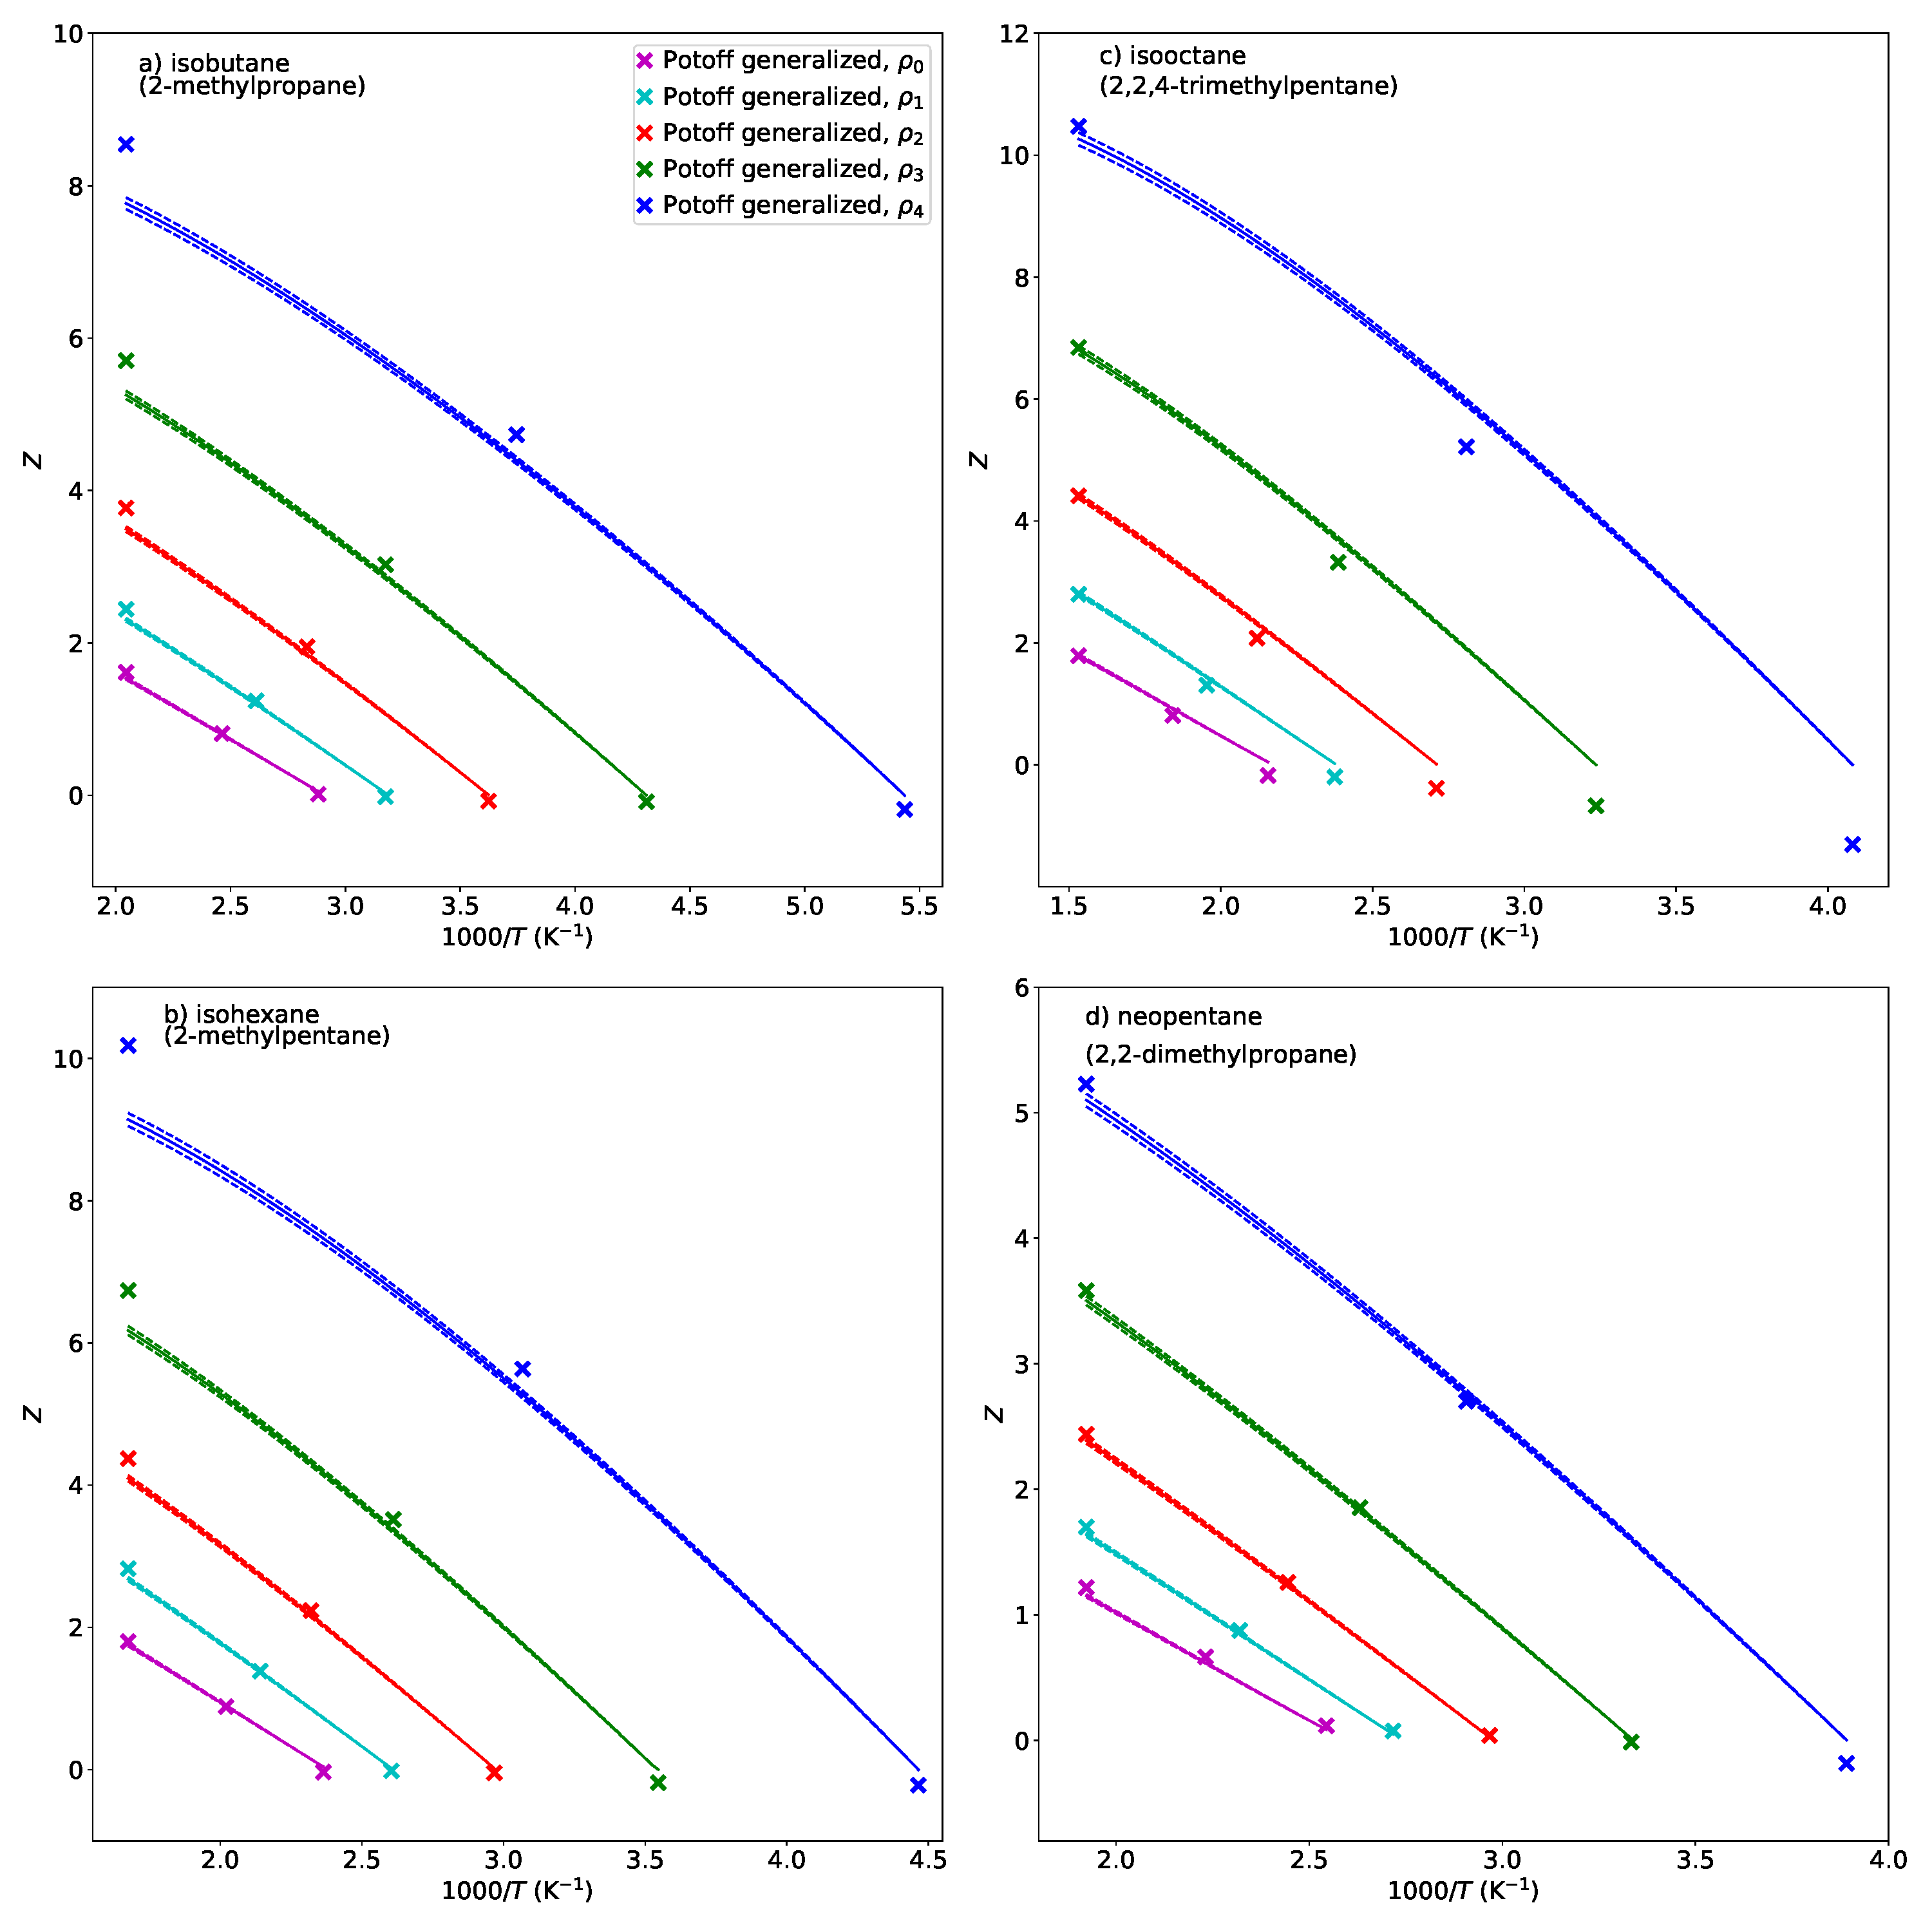
\includegraphics[width=6.2in]{IC_branched_alkanes_supporting_information}
	\caption{Compressibility factors $(Z)$ along isochores for branched alkanes deviate strongly at higher pressures using the Potoff generalized force field. Panels a)-d) correspond to isobutane, isohexane, isooctane, and neopentane, respectively. Symbols, lines, uncertainties, and formatting are the same as those in Figure \ref{fig:IC_normal_alkanes}.}
	\label{fig:IC_branched_alkanes_supporting_information}
\end{figure}

\newpage

\section{MCMC Example} \label{MCMC Example}

In this section we present typical results from an MCMC run. All of the MCMC runs performed in this study used 10000 MCMC steps for the burn-in period and an additional 10000 MCMC steps for the production period. The proposal distribution variances $(s^2_{\epsilon}$ and $s^2_{\sigma})$ were tuned every 100 MCMC steps during the burn-in period. Specifically, if the acceptance ratio was less than 20\%, the variances were decreased by a factor $0.9^2$. If the acceptance ratio was greater than 50\%, the variances were increased by a factor of $1.1^2$. During the production period, every 20 MCMC steps are stored to account for auto-correlation. Thus, the posterior predictive results for $\rho_{\rm l, MCMC}^{\rm sat}$, $P_{\rm v, MCMC}^{\rm sat}$, and $Z_{\rm MCMC}$ are based on 500 $\epsilon_{\rm MCMC}$--$\sigma_{\rm MCMC}$ parameter sets. 

Figures \ref{fig:MCMC_supporting_information}-\ref{fig:MCMC_supporting_information_2} provide an example of the MCMC results for ethane with $\lambda_{\rm CH_3} = 16$. Figure \ref{fig:MCMC_supporting_information} Panels a)-c) demonstrate that a burn-in period of 10000 steps is sufficient for an ergodic-like sampling of $\sigma$, $\epsilon$ and $\log(Pr)$, respectively. Panels d)-e) show that the respective distributions for $\sigma$ and $\epsilon$ appear to be normal. Note that the histograms of Panels d)-f) only include production period samples. The acceptance rate for proposed moves in $\epsilon$ and $\sigma$ was 28.8\%. 

\begin{figure}[p!]
	\centering
	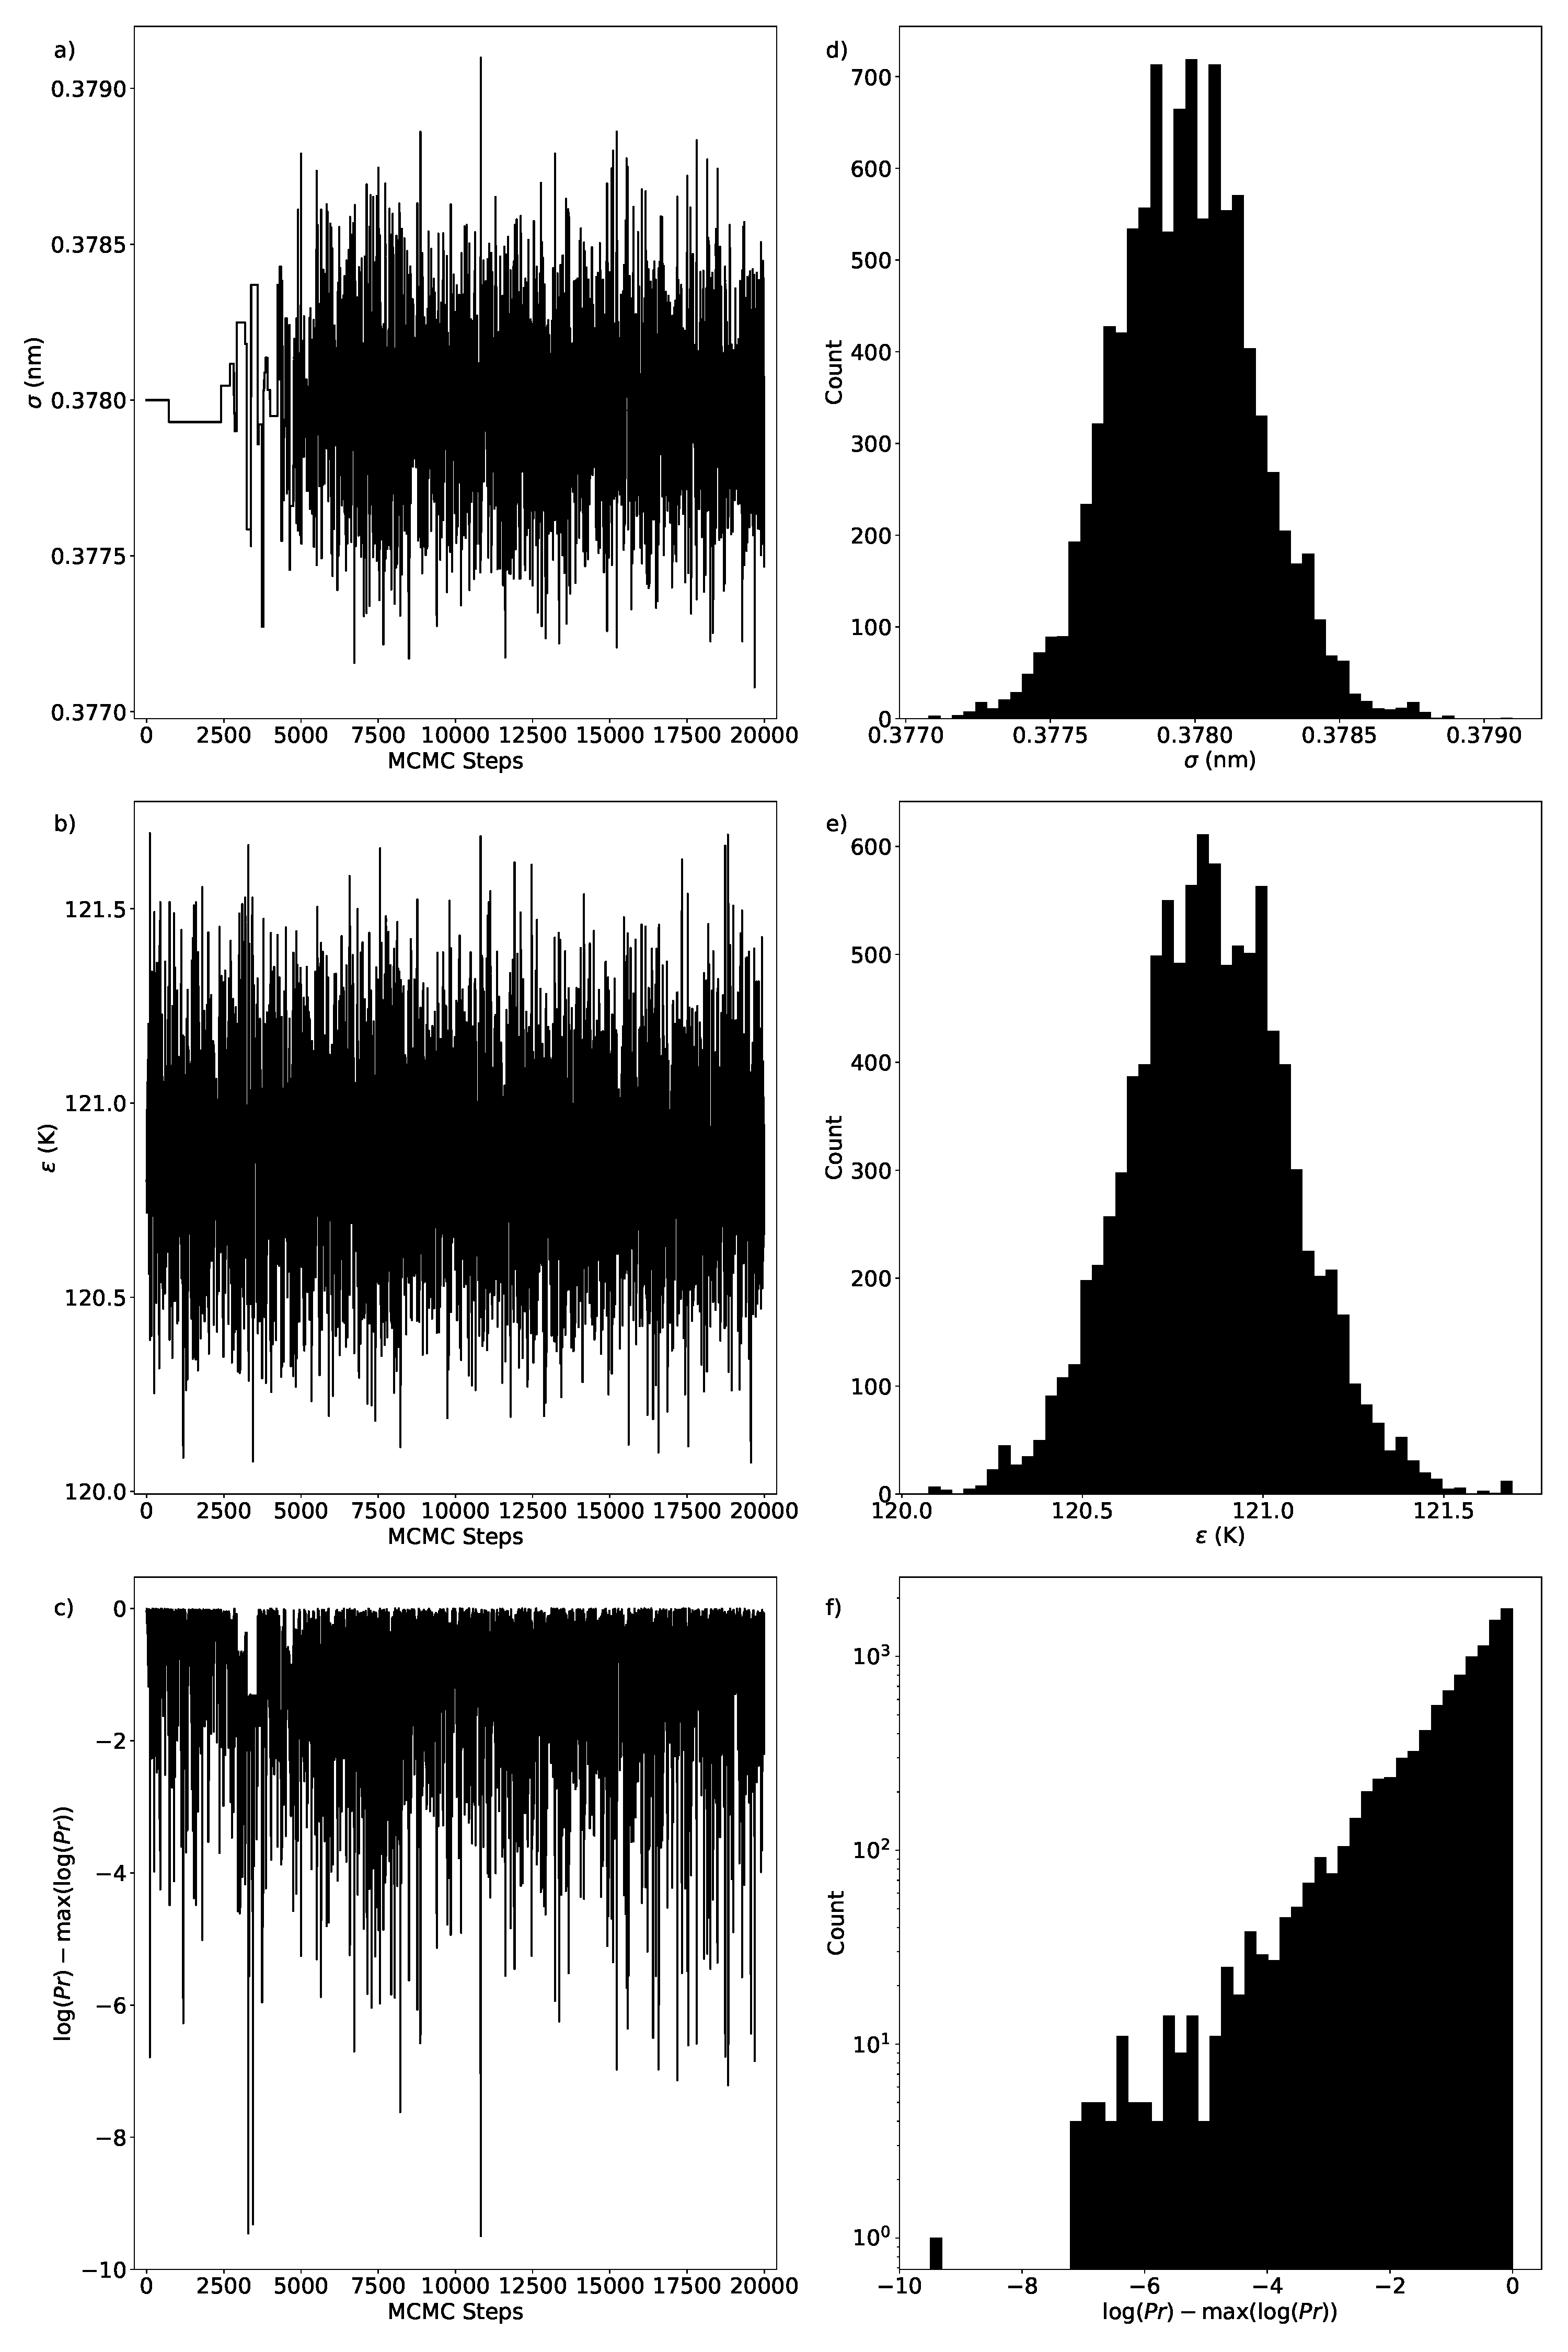
\includegraphics[width=5.4in]{MCMC_supporting_information}
	\caption{Panels a)-c) plot the respective traces of $\sigma$, $\epsilon$ and $\log(Pr)$, where $Pr$ is the posterior. Panels d)-f) plot histograms of the production period samples for $\sigma$, $\epsilon$ and $\log(Pr)$, respectively. Note that $\log(Pr)$ is normalized by the maximum $\log(Pr)$.}
	\label{fig:MCMC_supporting_information}
\end{figure} 

\newpage

\begin{figure}[p!]
	\centering
	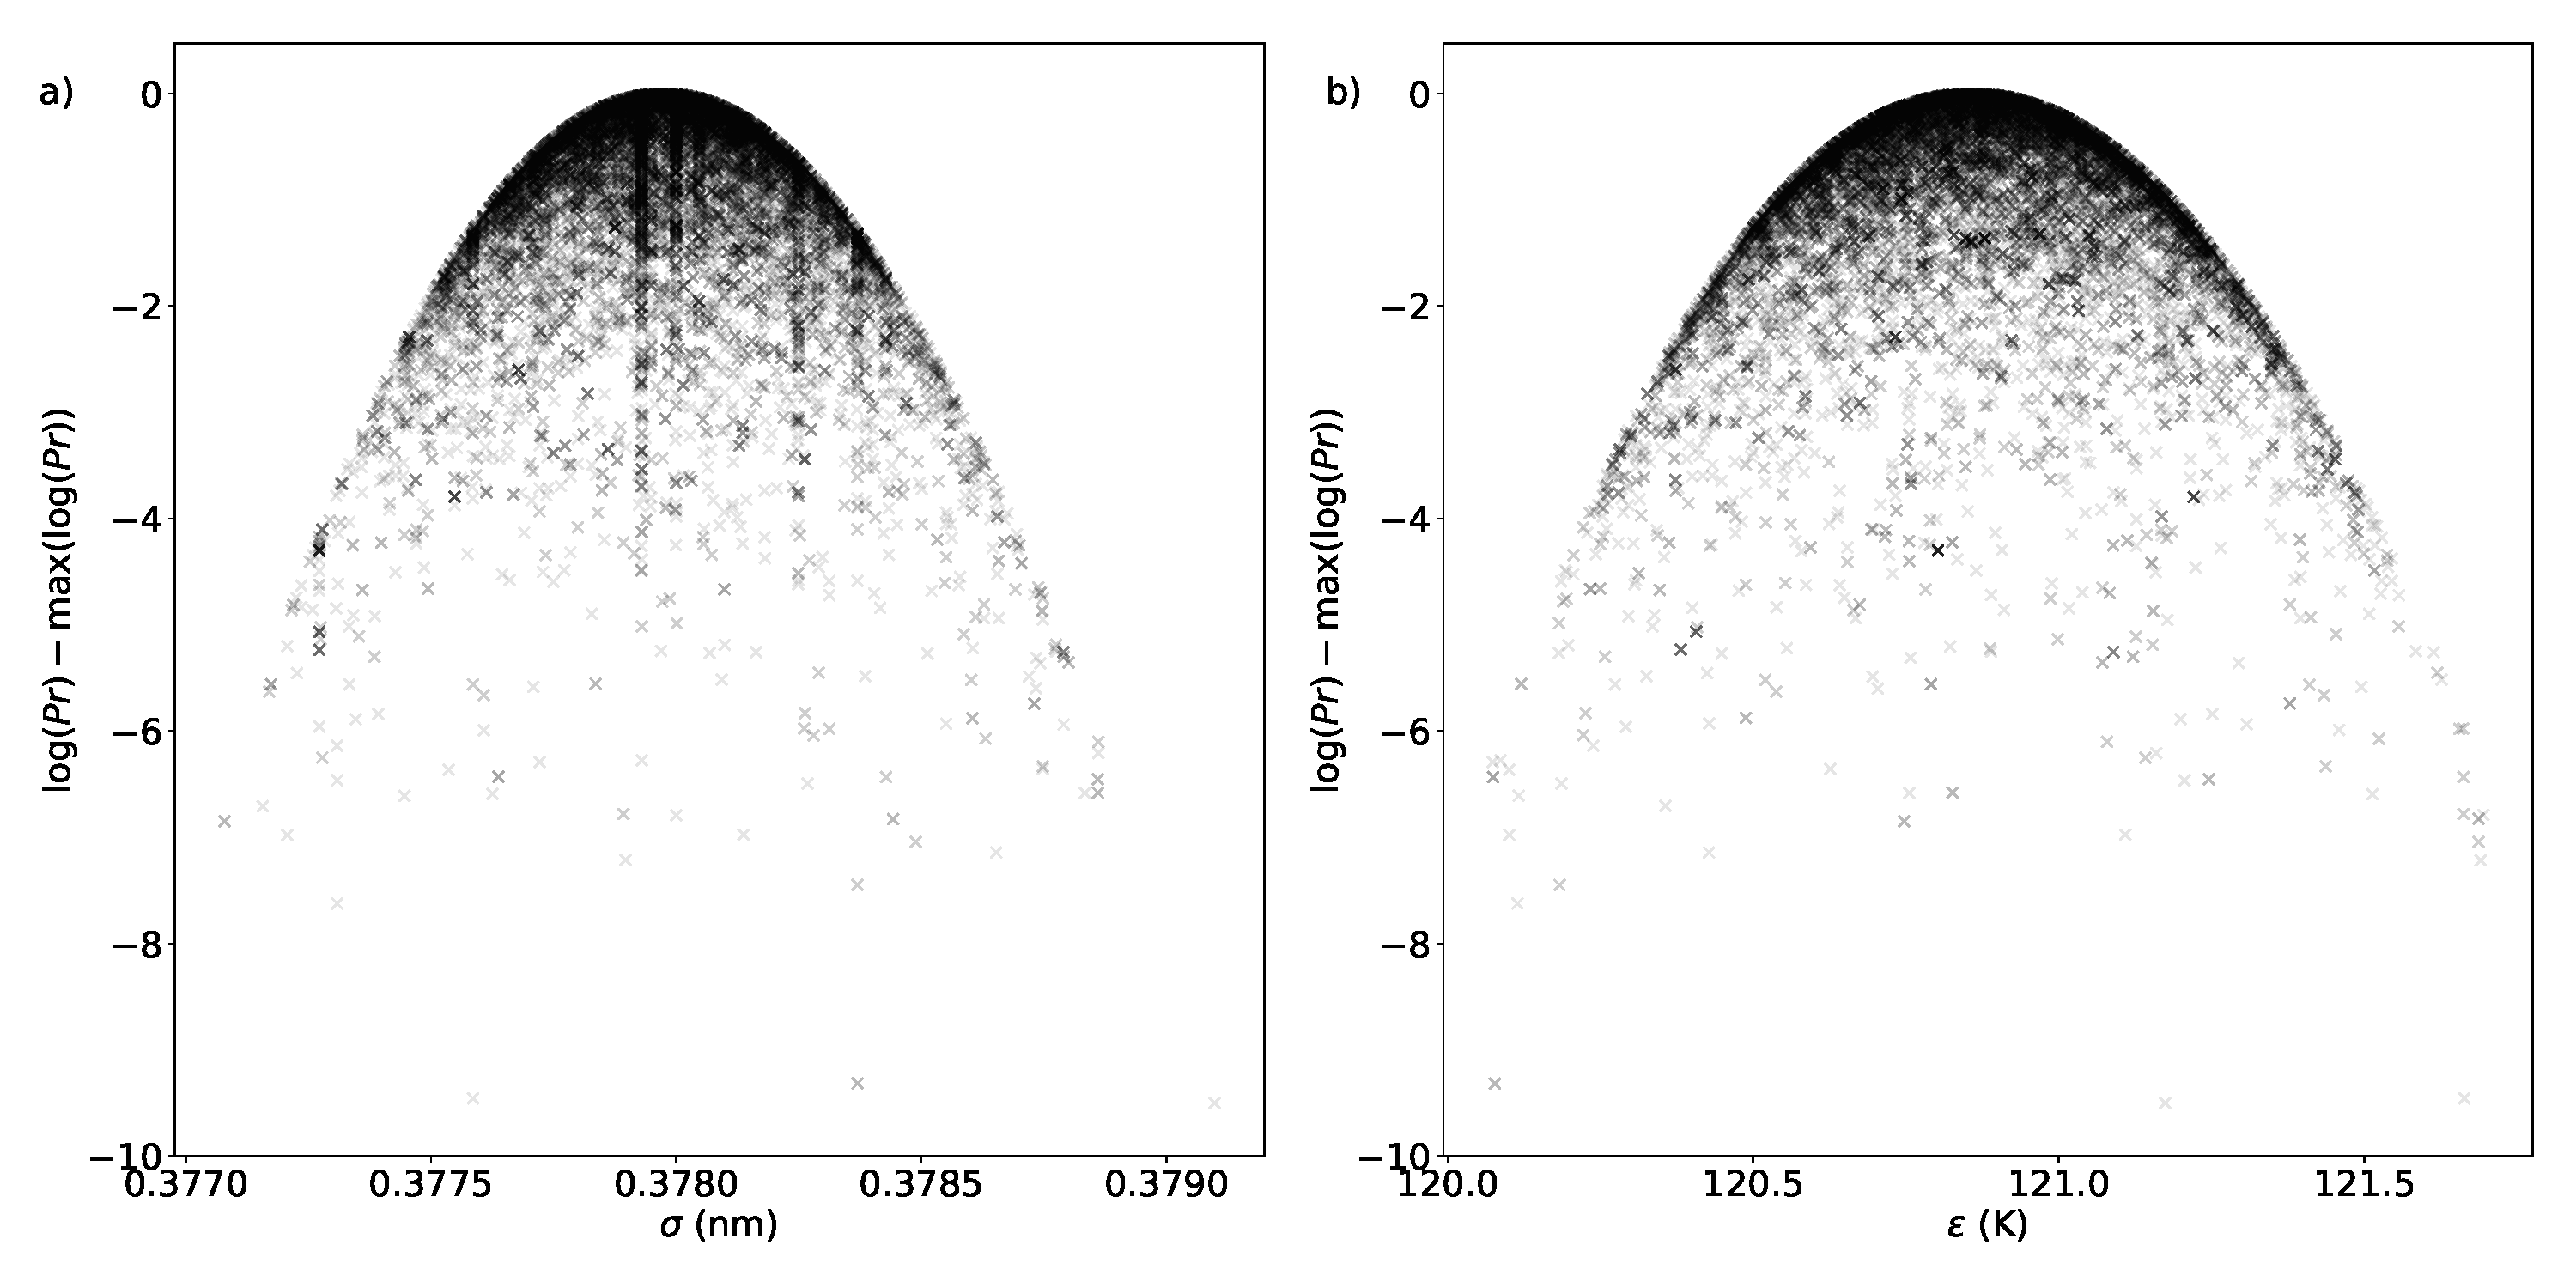
\includegraphics[width=6.4in]{MCMC_supporting_information_2}
	\caption{Panels a)-b) plot the dependence of $\log(Pr)$ (normalized by the maximum $\log(Pr)$, where $Pr$ is the posterior) with respect to $\sigma$ and $\epsilon$.}
	\label{fig:MCMC_supporting_information_2}
\end{figure} 

\newpage

\section{Additional Properties} \label{Udep and Z_IT}

Figure \ref{fig:MCMC_Mie_ZIT_alkanes} compares the MCMC results of different $\lambda$ values for $Z$ along the supercritical isotherms of the \textit{n}-alkanes studied. The purpose of this plot is to demonstrate deviations in the slope of $Z$ with respect to density for a constant temperature, i.e. $\left(\frac{\partial Z}{\partial \rho}\right)_T$, which is related to $A_{01}^{\rm dep}$ and $A_{02}^{\rm dep}$ (see Equation \ref{eq:Z_IT}). The deviations at high densities along the supercritical isotherm are already explained in the main text. For this reason, the insets focus on the low density region. Inset in Panel a) shows that the 13-6 potential under-predicts $Z$ at low density while it agrees well at high density. Recall that for ethane the 13-6 potential is very accurate at predicting $Z$ and even the slope of $Z$ along the isochores, i.e. $\left(\frac{-\partial Z}{\partial(1/T)}\right)_\rho$. However, the 13-6 potential does not appear to have the correct slope for $Z$ along the isotherm, i.e. $Z$ $\left(\frac{\partial Z}{\partial \rho}\right)_T$. The same trend is observed for the 14-6 potential in all four \textit{n}-alkanes, namely, the improvement for predicting $Z$ at high densities typicaly results in under-prediction of $Z$ at low densities.

\begin{figure}[p!]
	\centering
	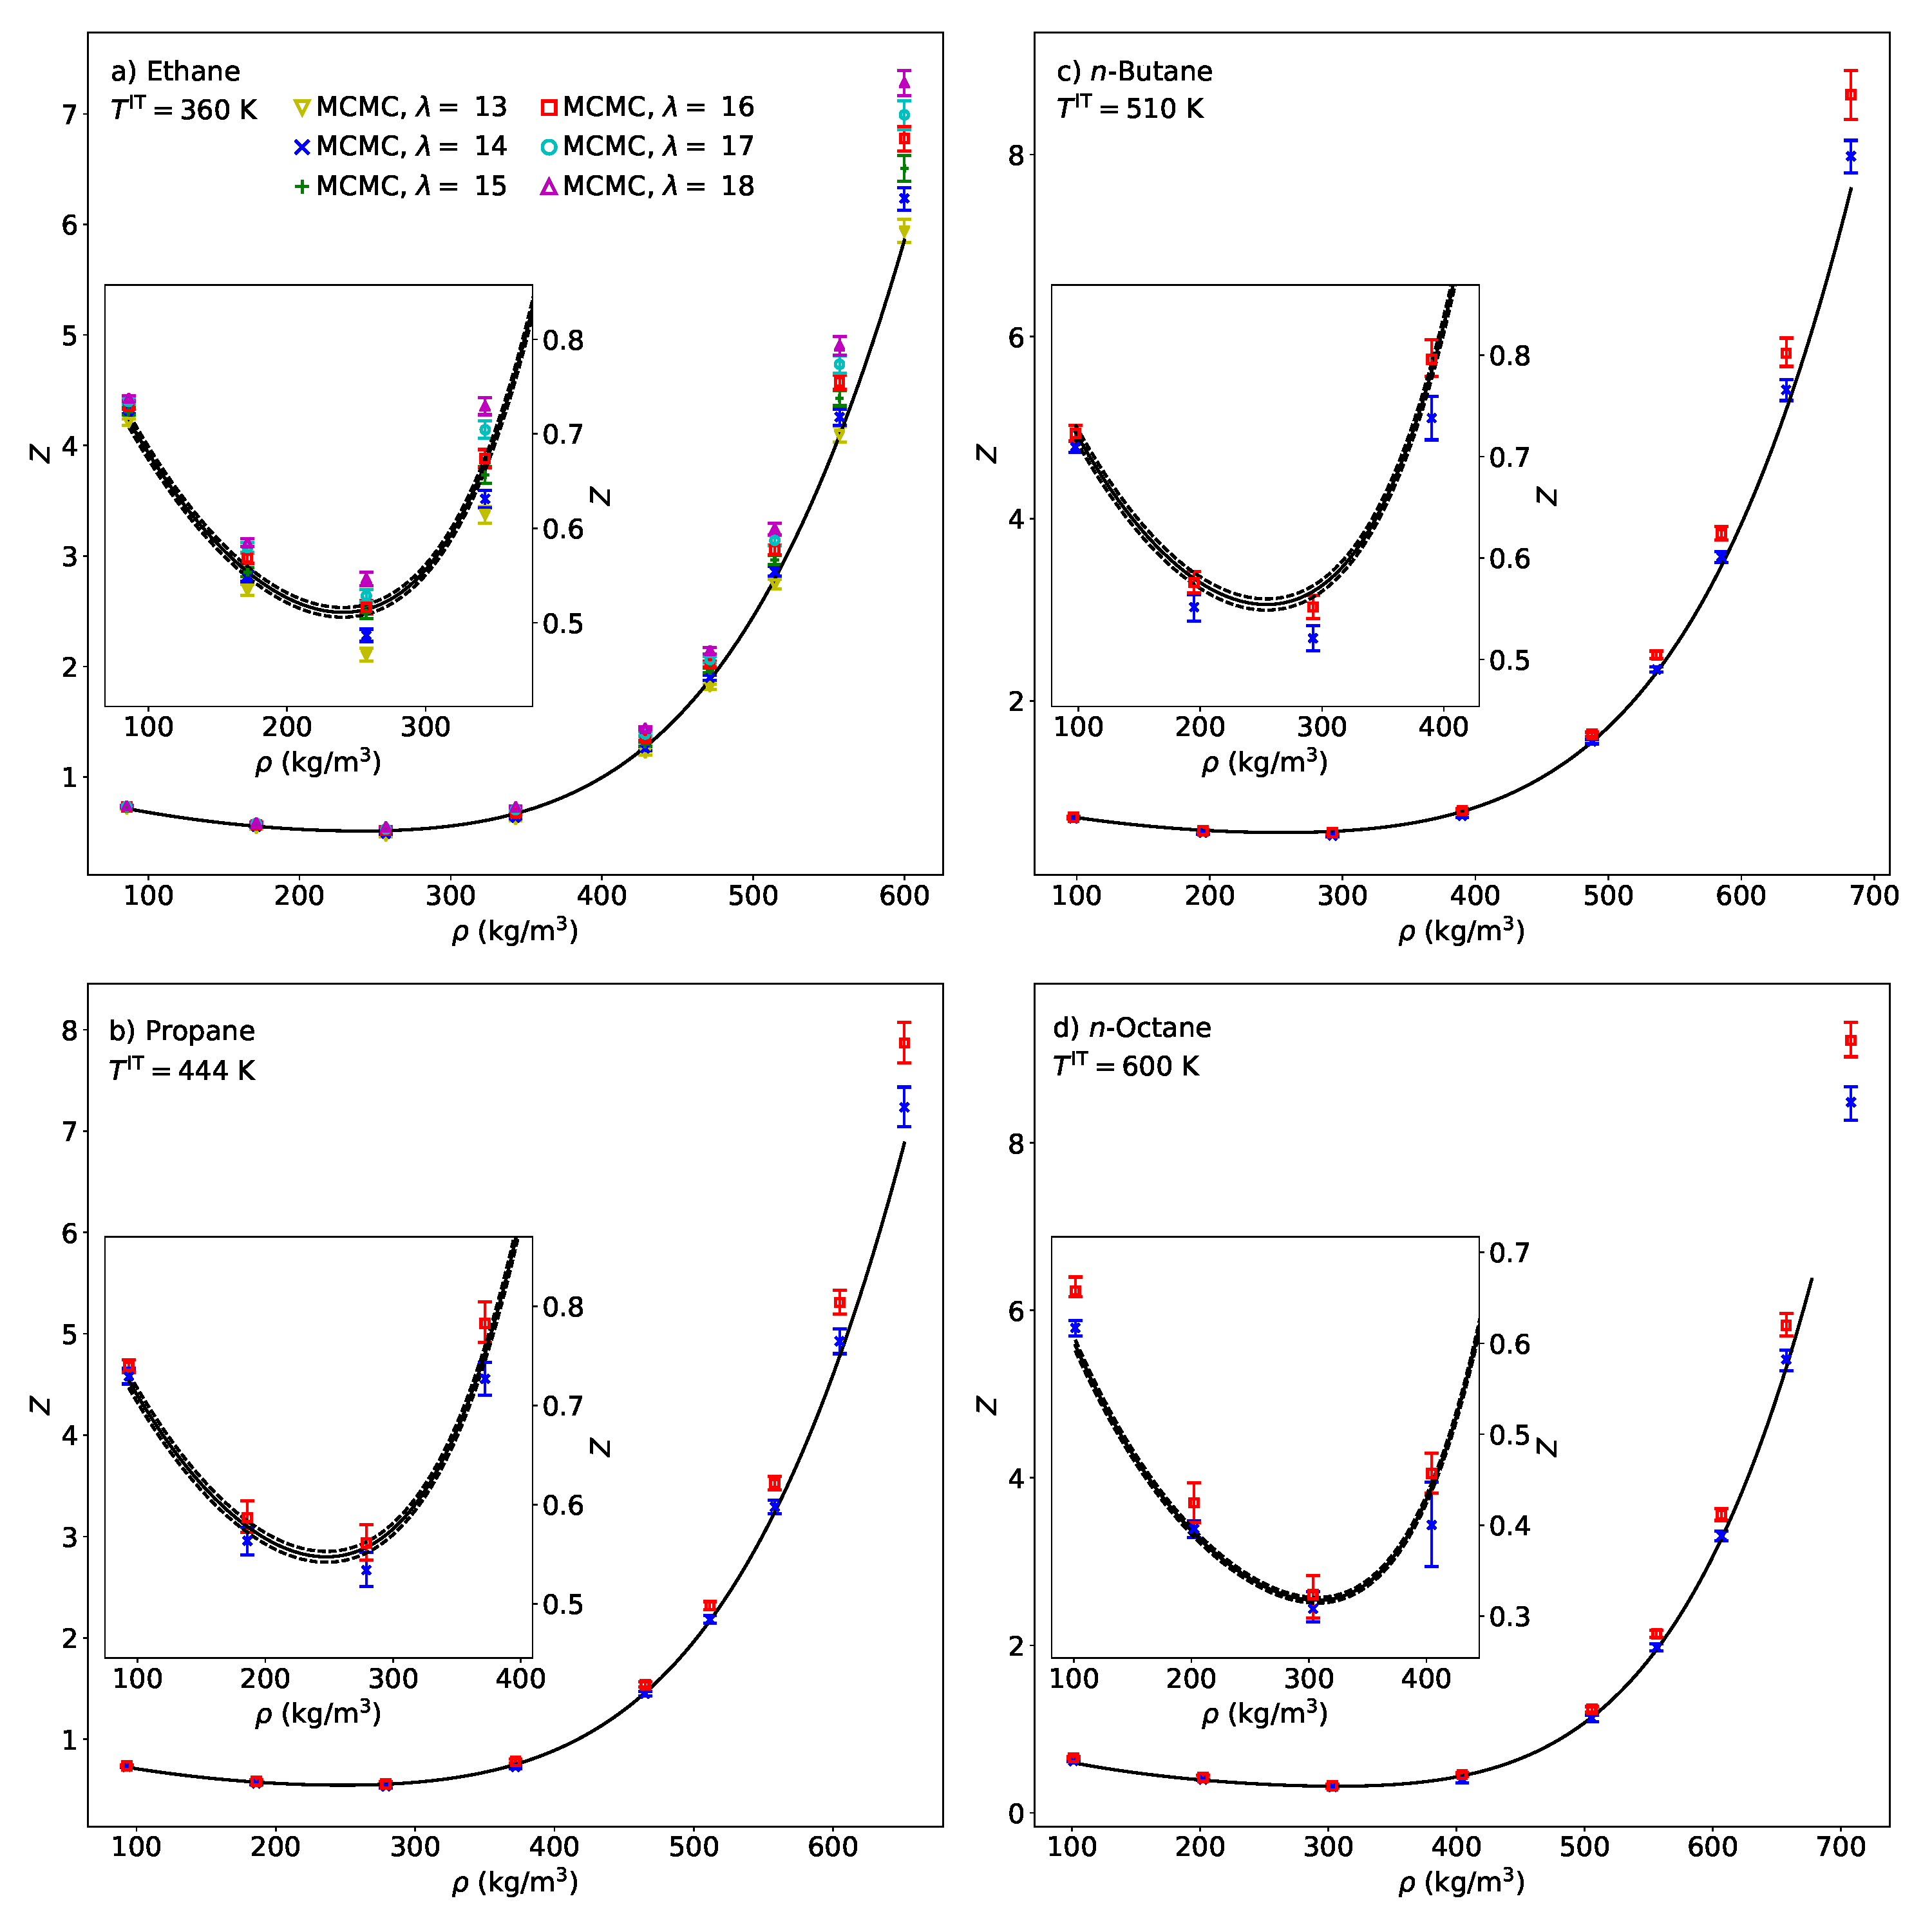
\includegraphics[width=6.4in]{MCMC_Mie_ZIT_alkanes}
	\caption{$Z_{\rm MCMC}$ along the supercritical isotherms for different $\lambda$ values. Panels a)-d) correspond to ethane, propane, \textit{n}-butane, and \textit{n}-octane, respectively. Solid lines are the REFPROP correlation with dashed lines (included only in the insets) representing a 1\% uncertainty.}
	\label{fig:MCMC_Mie_ZIT_alkanes}
\end{figure} 

Figure \ref{fig:MCMC_Mie_UIC_alkanes} compare the MCMC results of different $\lambda$ values for $U^{\rm dep}$ along the isochores of the \textit{n}-alkanes studied. The purpose of this plot is to demonstrate deviations in $U^{\rm dep}$ and the slope of $U^{\rm dep}$ with respect to temperature for a constant density, i.e. $\left(\frac{\partial U^{\rm dep}}{\partial T}\right)_\rho$, which are related to $A_{10}^{\rm dep}$ and $A_{20}^{\rm dep}$, respectively (see Equations \ref{eq:U}-\ref{eq:U_IC}). Definitive conclusions are difficult due to the relatively large uncertainty in the REFPROP correlations, approximated to be 5\%. However, Panel a) demonstrates that at $T^{\rm sat}$, i.e. the lowest temperature for a given isochore, $\lambda = 15$ accurately predicts $U^{\rm dep}$ while $\lambda > 15$ and $\lambda < 15$ consistently under- and over-predict $U^{\rm dep}$ at $T^{\rm sat}$. By contrast, $\lambda = 13$ agrees more closely with $U^{\rm dep}$ at $T^{\rm IT}$, i.e. the highest temperature, while $\lambda > 13$ under-predict $U^{\rm dep}$ at $T^{\rm IT}$. A similar trend is observed for propane, \textit{n}-butane, and \textit{n}-octane, namely, $\lambda = 16$ and $\lambda = 14$ are more accurate at $T^{\rm sat}$ and $T^{\rm IT}$, respectively. These results suggest that all values of $\lambda$ are inaccurate for $\left(\frac{\partial U^{\rm dep}}{\partial T}\right)_\rho$ and are only reliable for $U^{\rm dep}$ at certain conditions. Note that the isochoric heat capacity is directly related to $\left(\frac{\partial U^{\rm dep}}{\partial T}\right)_\rho$.

\begin{figure}[p!]
	\centering
	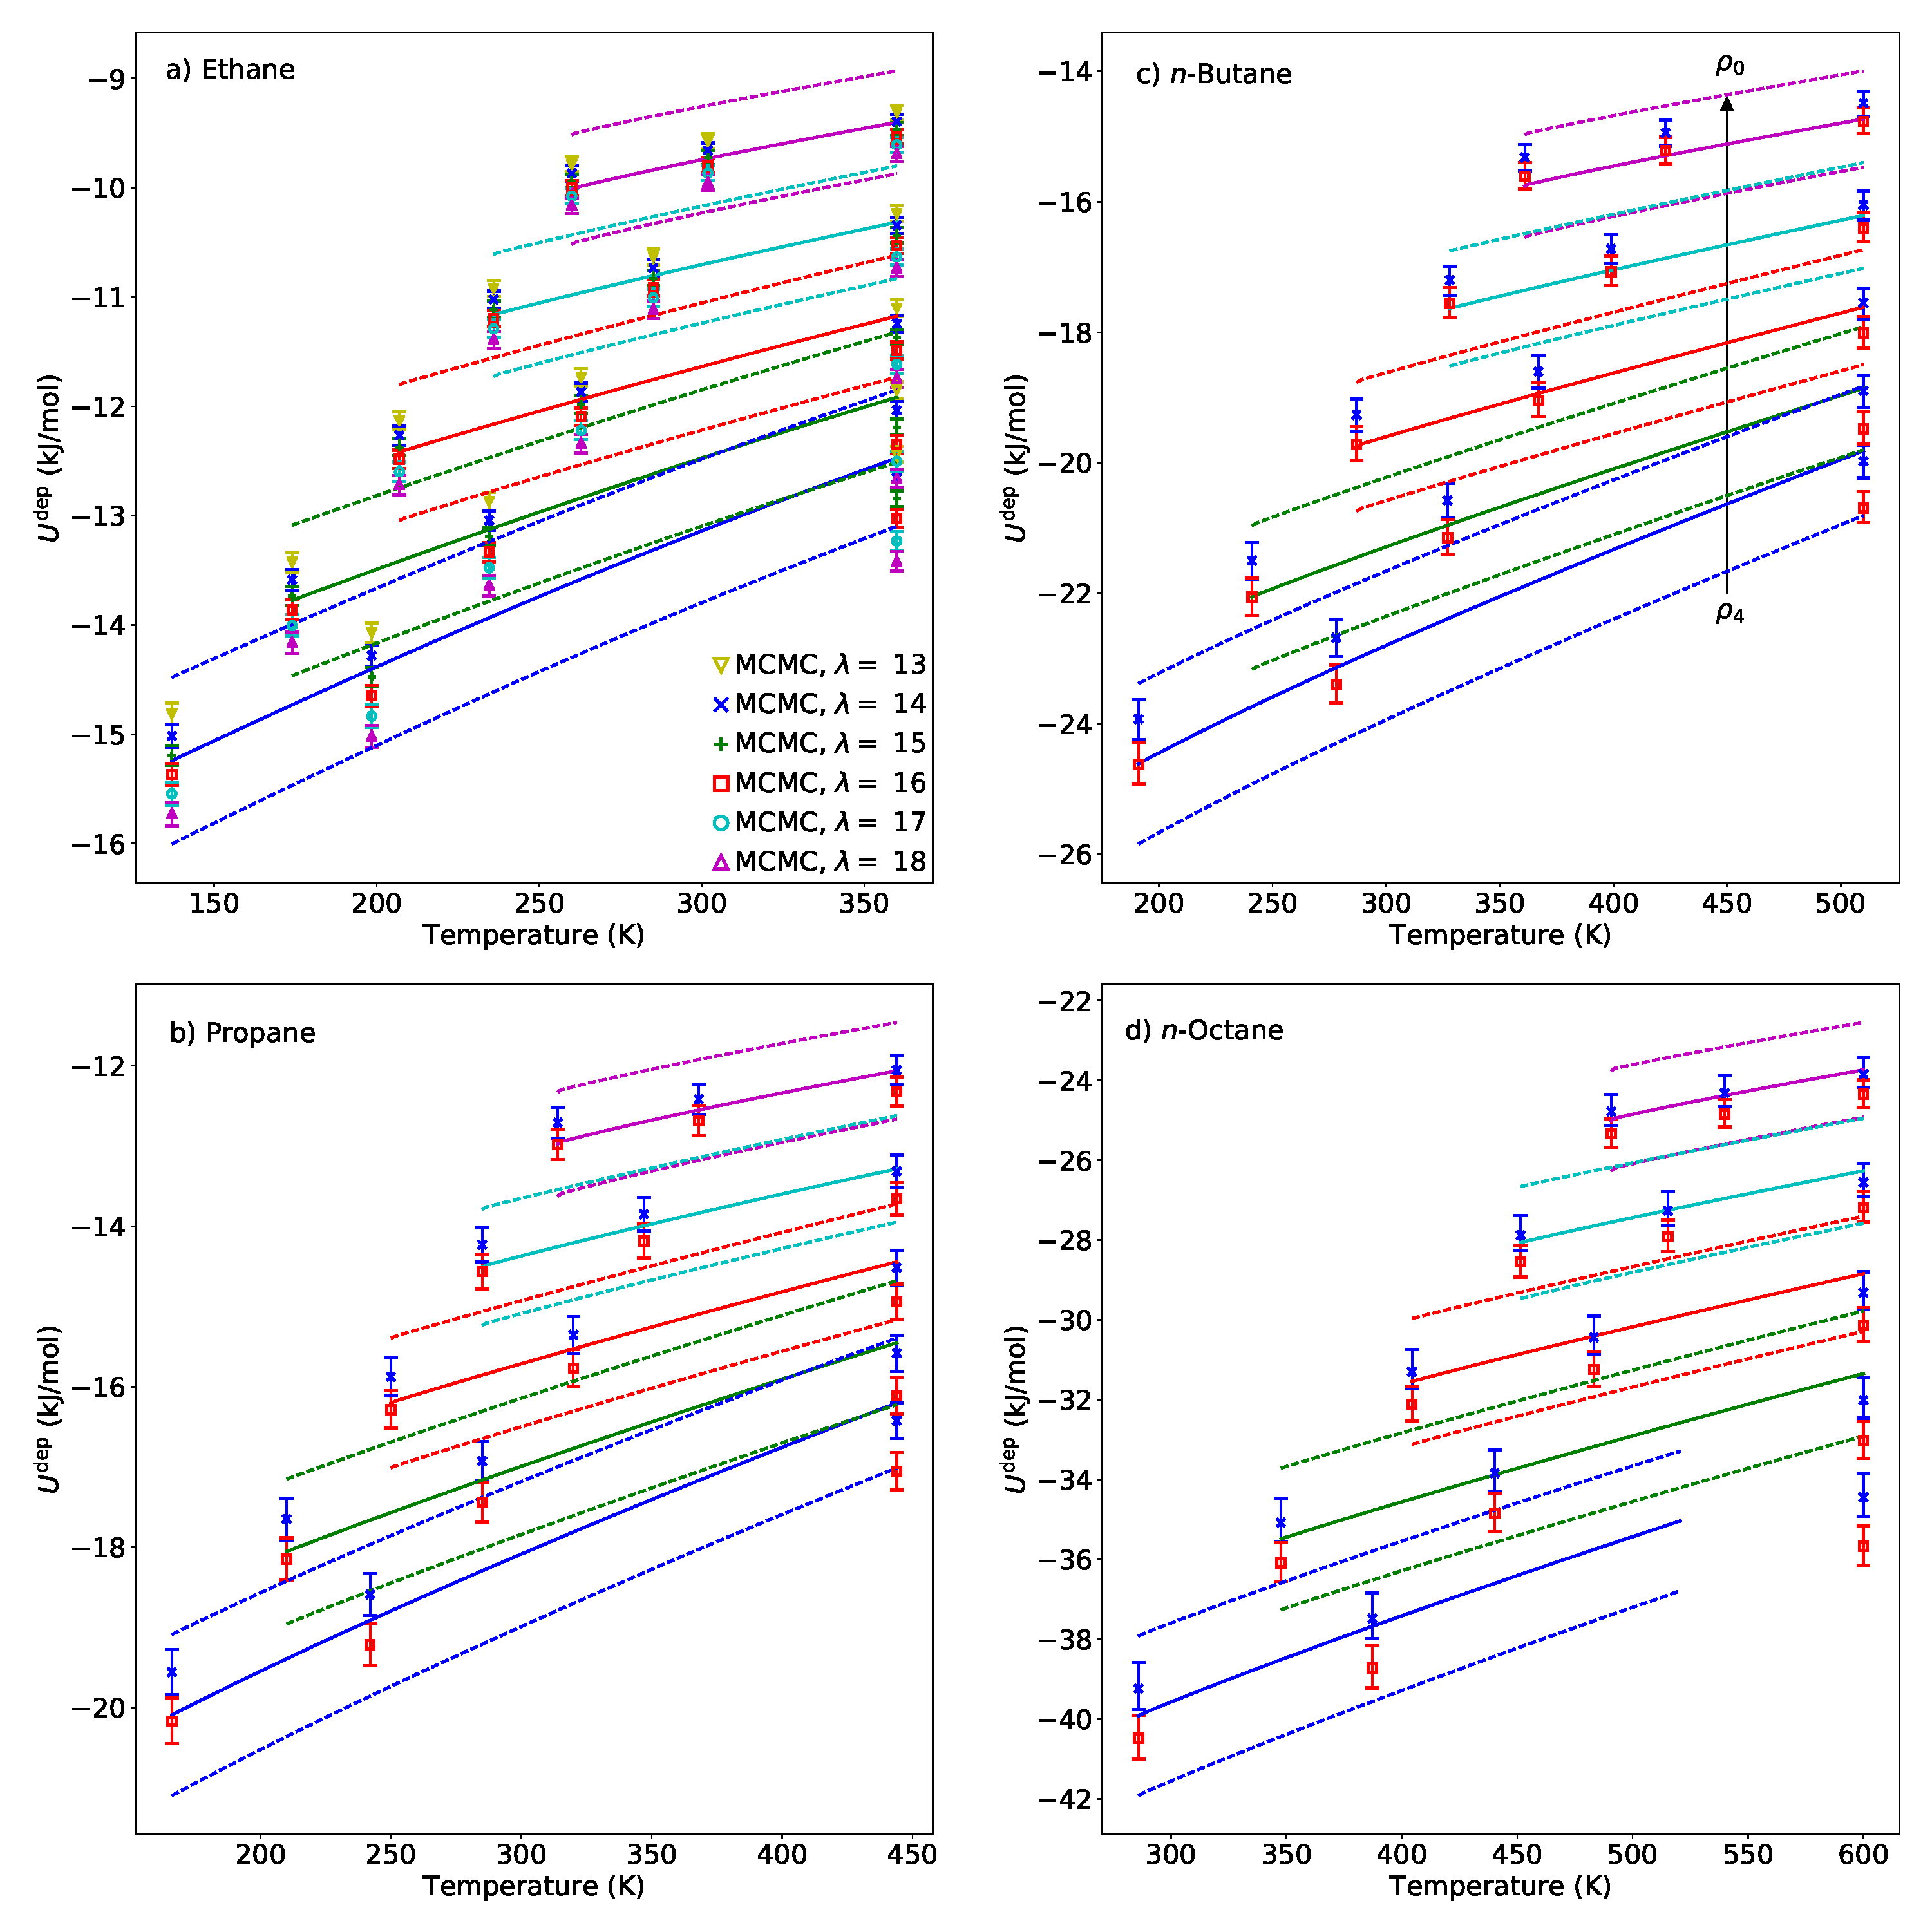
\includegraphics[width=6.4in]{MCMC_Mie_UIC_alkanes}
	\caption{$U^{\rm dep}_{\rm MCMC}$ along the isochores for different $\lambda$ values. Panels a)-d) correspond to ethane, propane, \textit{n}-butane, and \textit{n}-octane, respectively. Solid lines are the REFPROP correlation with dashed lines representing a 5\% uncertainty. Line colors of different isochores correspond with Figures \ref{fig:IC_normal_alkanes}-\ref{fig:IC_branched_alkanes} in main text.}
	\label{fig:MCMC_Mie_UIC_alkanes}
\end{figure} 

\newpage

\section{Error Model} \label{Error Model}

Figure \ref{fig:ITIC_validation_error_model} presents the percent deviation between the surrogate model $(\rm SM)$ and literature $(\rm lit)$ VLE values using the TraPPE-UA and Potoff force fields for ethane, propane, \textit{n}-butane, and \textit{n}-octane. From this figure, an approximate surrogate model uncertainty was deduced such that most of the points, with their corresponding error bars, would lie within this uncertainty region. Note that the majority of literature values are for $T_r > 0.6$, therefore, we used our best judgment when extrapolating the surrogate model uncertainties to $T_r = 0.45$. 

\begin{figure}[p!]
	\centering
	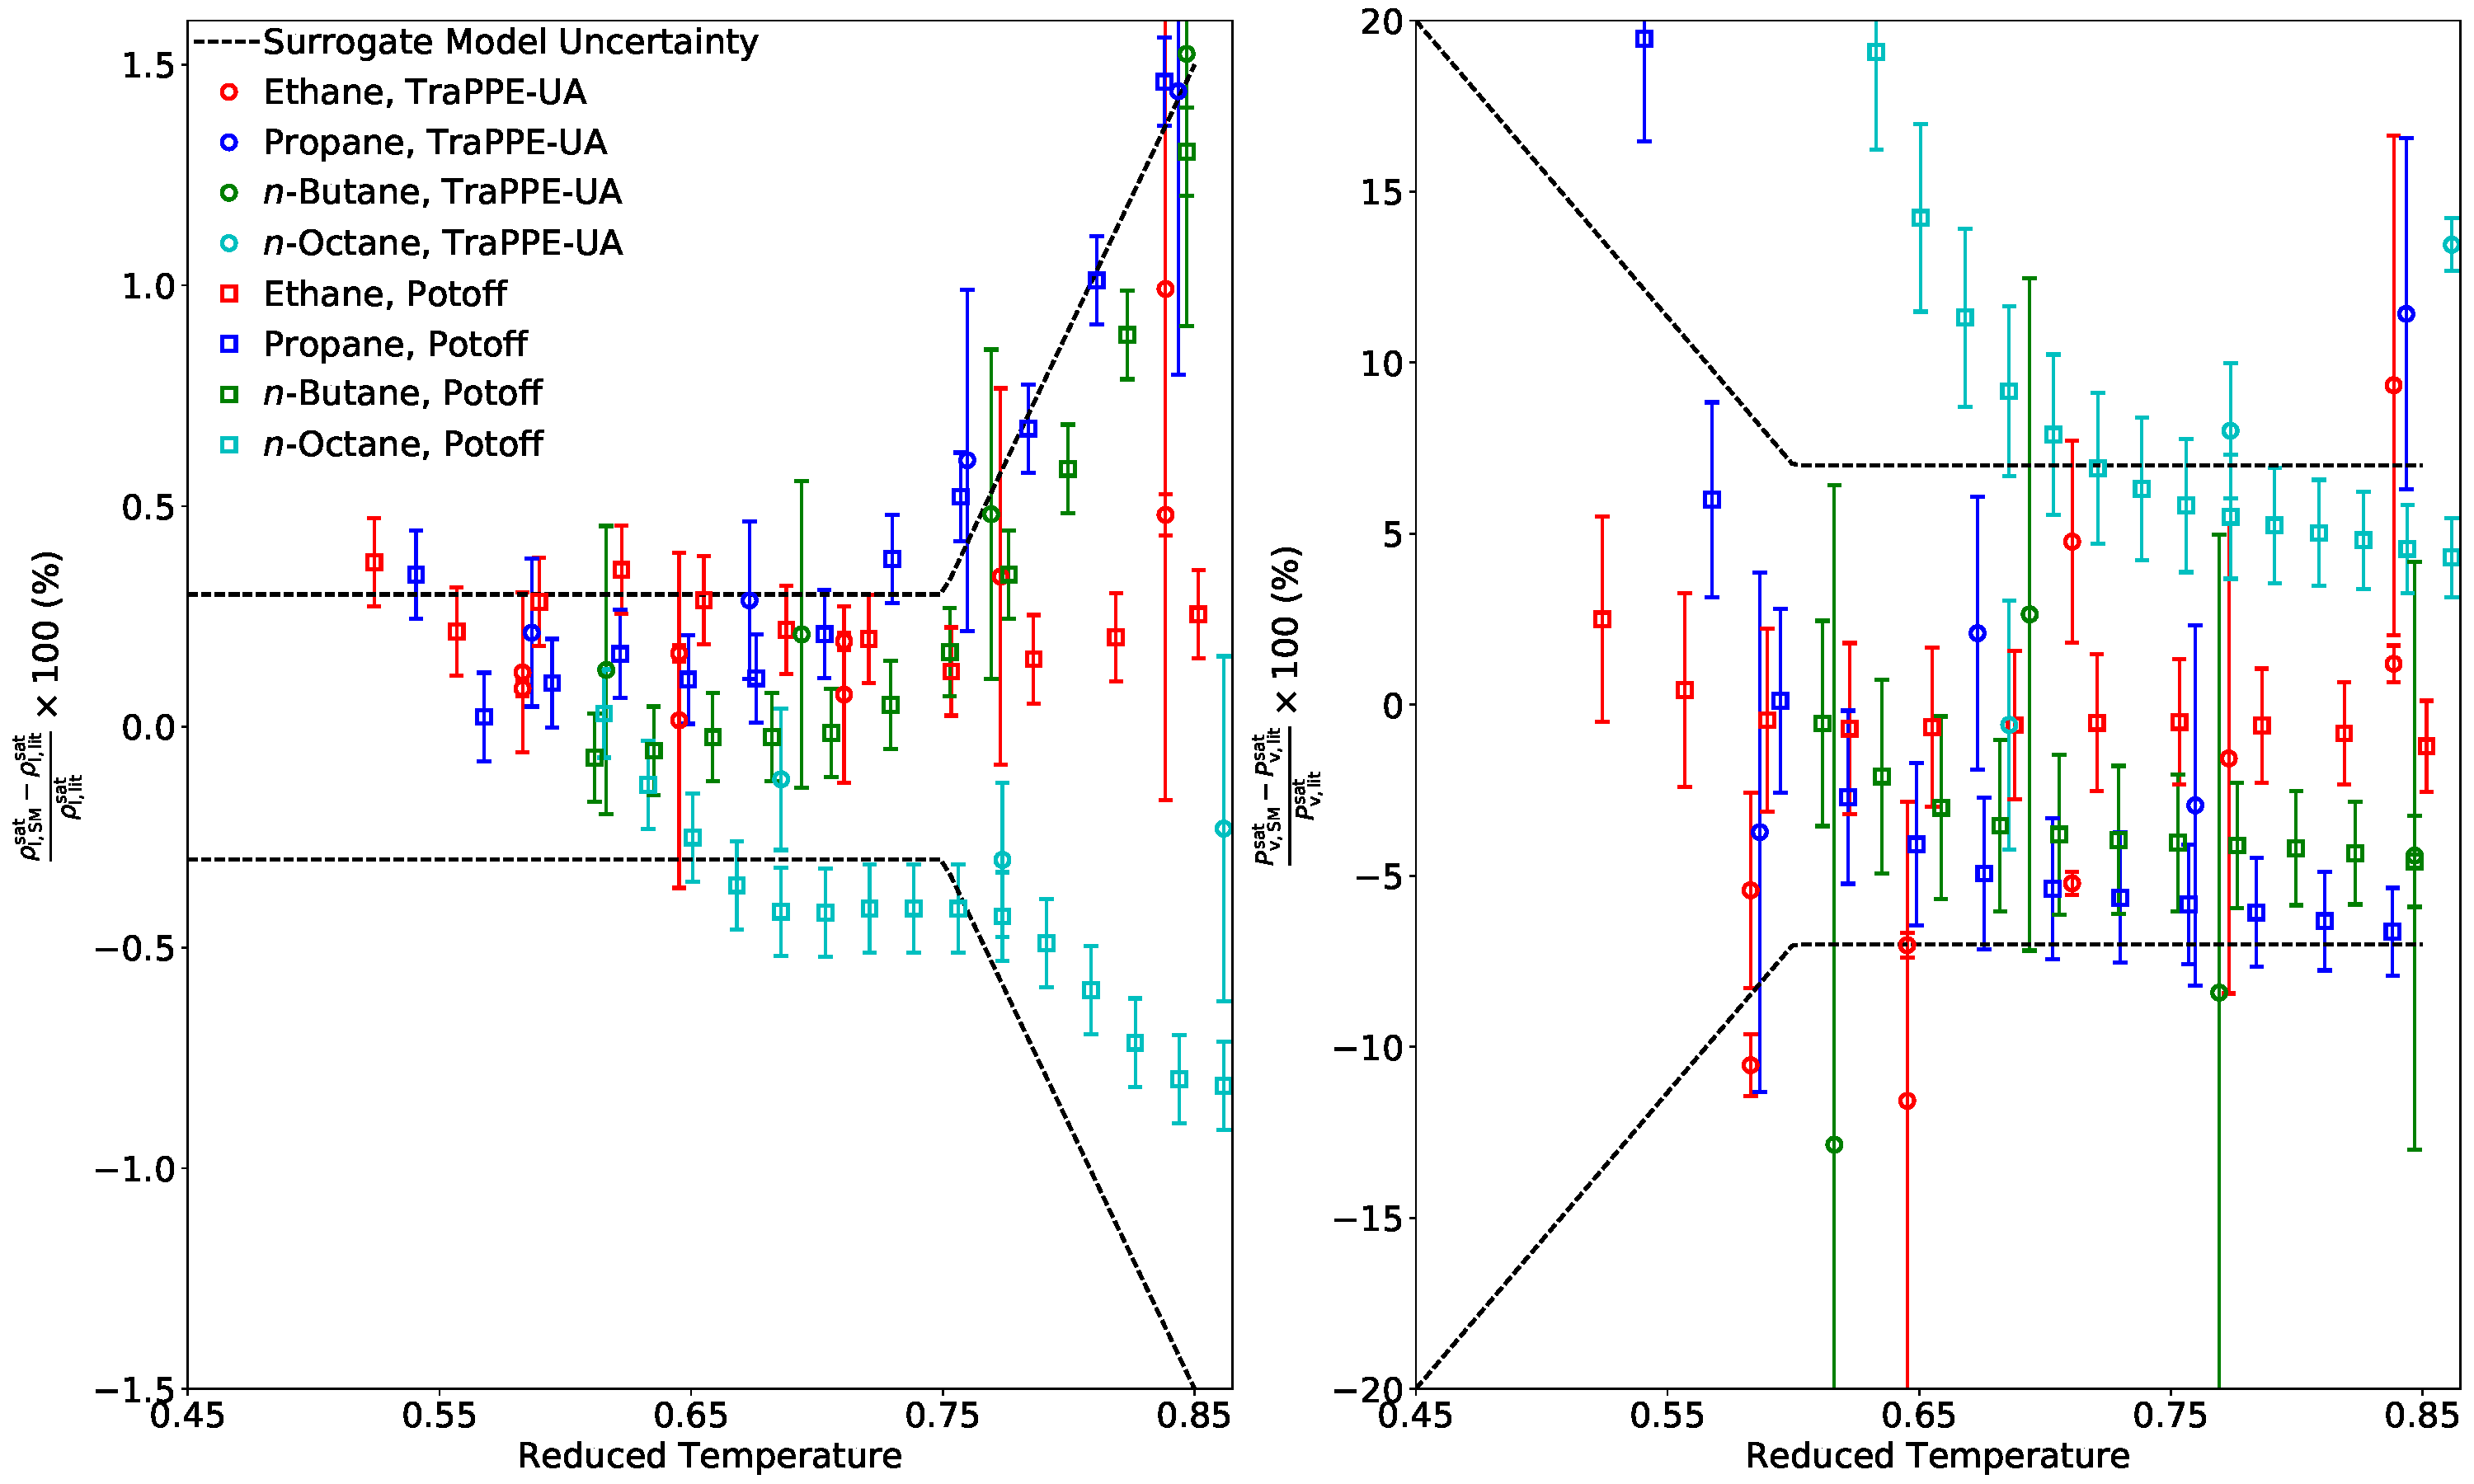
\includegraphics[width=6.4in]{ITIC_validation_error_model}
	\caption{Panels a)-b) demonstrate how well the surrogate model uncertainty agrees with the percent deviations between the surrogate model and literature values for $\rho_{\rm l}^{\rm sat}$ and $P_{\rm v}^{\rm sat}$, respectively. Reduced temperature is relative to the REFPROP $T_c$. The TraPPE-UA and Potoff literature values were obtained using GEMC \cite{TraPPE,Validation} and GCMC \cite{Mie}, respectively. Error bars represent statistical uncertainties that were obtained using replicate simulations. The error bars for TraPPE-UA were obtained from References \citenum{TraPPE,Validation}, or alternatively on the TraPPE website. No attempt was made to determine if these are standard deviations or 95\% confidence intervals. The error bars for the Potoff model are a constant 0.1\% for $\rho_{\rm l}^{\rm sat}$ and 0.5-3\% for $P_{\rm v}^{\rm sat}$, increasing linearly with decreasing reduced temperature. The values 0.5-3\% were reported in Reference \citenum{Mie}. As Reference \citenum{Mie} did not report uncertainties for $\rho_{\rm l}^{\rm sat}$, the value of 0.1\% is based on some of Potoff's more recent work. \cite{Potoff_branched}}
	\label{fig:ITIC_validation_error_model}
\end{figure} 

There are two likely reasons to explain why the percent deviations in $\rho_{\rm l}^{\rm sat}$ increase with respect to temperature. First, ITIC neglects the higher order virial terms that become more important at higher temperatures. Second, we use the REFPROP $B_2$ and $B_3$ values, rather than those of the force field. By contrast, the larger percent deviations in $P_{\rm v}^{\rm sat}$ with decreasing temperature are attributed primarily to the difference in orders of magnitude for $P_{\rm v}^{\rm sat}$, since the virial coefficients should not impact $P_{\rm v}^{\rm sat}$ at lower temperatures.  

Aside from these expected trends, some other unexplained deviation trends are observed for a specific property, compound, and/or force field. However, it is not readily obvious if these deviations are caused by limitations in the surrogate model or the literature values themselves. For example, the TraPPE-UA and Potoff literature values were obtained using GEMC \cite{TraPPE,Validation} and GCMC \cite{Mie}, respectively. These Monte Carlo methods can suffer from low insertion acceptance at $T_r<0.7$, which can result in erroneous VLE values, for $P_{\rm v}^{\rm sat}$ in particular. It is not our intention to imply that our values are better than either the TraPPE-UA or Potoff literature values, but rather we wish to emphasize that it should be expected that our approach would not yield exactly the same values as other methods. It is for this precise reason that our surrogate model uncertainty is larger than the statistical uncertainties which are typically reported in the literature.  

\newpage

\bibliography{postdoc_references}

%\nobibliography{H:/Publications/Postdoc_3/postdoc_references.bib}{}

\end{document}